\subsection{Strucure locale et distribuée}
Comme nous l'avons vu dans la section précédente, les automates industriels sont reliés aux capteurs et pré-actionneurs du système.

Sur les systèmes de petite taille et si l'installation le permet, les entrées et sorties de l'automate sont reliées directement à l'automate, on parle de \textbf{structure locale}. Pour des installations plus grande ou lorsque la configuration l'impose, les entrées et sorties sont reliées à des modules déportés (éloignés de l'automate), on parle de \textbf{structure déportée}. Ces deux configurations sont illustrée sur la Figure~\ref{fig:local_deporte}

\begin{figure}[h]
	\begin{subfigure}[b]{.49\textwidth}
		\centering
		


\tikzset{every picture/.style={line width=0.75pt}} %set default line width to 0.75pt

\begin{tikzpicture}[x=0.75pt,y=0.75pt,yscale=-1,xscale=1]
%uncomment if require: \path (0,300); %set diagram left start at 0, and has height of 300

%Image [id:dp060131966756508004]
\draw (75,57) node  {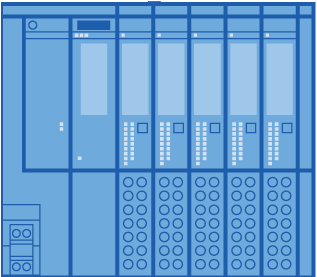
\includegraphics[width=52.5pt,height=52.5pt]{images/siemens_schema.png}};
%Rounded Rect [id:dp7545427239837935]
\draw   (47,129.03) .. controls (47,124.59) and (50.59,121) .. (55.03,121) -- (120.57,121) .. controls (125.01,121) and (128.6,124.59) .. (128.6,129.03) -- (128.6,153.11) .. controls (128.6,157.54) and (125.01,161.13) .. (120.57,161.13) -- (55.03,161.13) .. controls (50.59,161.13) and (47,157.54) .. (47,153.11) -- cycle ;
%Straight Lines [id:da21237841433953675]
\draw [color={rgb, 255:red, 65; green, 117; blue, 5 }  ,draw opacity=1 ]   (71,92) -- (71,119) ;
\draw [shift={(71,121)}, rotate = 270] [color={rgb, 255:red, 65; green, 117; blue, 5 }  ,draw opacity=1 ][line width=0.75]    (10.93,-3.29) .. controls (6.95,-1.4) and (3.31,-0.3) .. (0,0) .. controls (3.31,0.3) and (6.95,1.4) .. (10.93,3.29)   ;

%Straight Lines [id:da9289871961779934]
\draw [color={rgb, 255:red, 208; green, 2; blue, 27 }  ,draw opacity=1 ]   (66,121) -- (66,94) ;
\draw [shift={(66,92)}, rotate = 450] [color={rgb, 255:red, 208; green, 2; blue, 27 }  ,draw opacity=1 ][line width=0.75]    (10.93,-3.29) .. controls (6.95,-1.4) and (3.31,-0.3) .. (0,0) .. controls (3.31,0.3) and (6.95,1.4) .. (10.93,3.29)   ;

%Straight Lines [id:da38366242506499526]
\draw [color={rgb, 255:red, 65; green, 117; blue, 5 }  ,draw opacity=1 ]   (104,92) -- (104,119) ;
\draw [shift={(104,121)}, rotate = 270] [color={rgb, 255:red, 65; green, 117; blue, 5 }  ,draw opacity=1 ][line width=0.75]    (10.93,-3.29) .. controls (6.95,-1.4) and (3.31,-0.3) .. (0,0) .. controls (3.31,0.3) and (6.95,1.4) .. (10.93,3.29)   ;

%Straight Lines [id:da1458665129852148]
\draw [color={rgb, 255:red, 208; green, 2; blue, 27 }  ,draw opacity=1 ]   (99,121) -- (99,94) ;
\draw [shift={(99,92)}, rotate = 450] [color={rgb, 255:red, 208; green, 2; blue, 27 }  ,draw opacity=1 ][line width=0.75]    (10.93,-3.29) .. controls (6.95,-1.4) and (3.31,-0.3) .. (0,0) .. controls (3.31,0.3) and (6.95,1.4) .. (10.93,3.29)   ;


%Straight Lines [id:da7281946578898251]
\draw [color={rgb, 255:red, 65; green, 117; blue, 5 }  ,draw opacity=1 ]   (88.5,92) -- (88.5,119) ;
\draw [shift={(88.5,121)}, rotate = 270] [color={rgb, 255:red, 65; green, 117; blue, 5 }  ,draw opacity=1 ][line width=0.75]    (10.93,-3.29) .. controls (6.95,-1.4) and (3.31,-0.3) .. (0,0) .. controls (3.31,0.3) and (6.95,1.4) .. (10.93,3.29)   ;

%Straight Lines [id:da7853722611490053]
\draw [color={rgb, 255:red, 208; green, 2; blue, 27 }  ,draw opacity=1 ]   (83.5,121) -- (83.5,94) ;
\draw [shift={(83.5,92)}, rotate = 450] [color={rgb, 255:red, 208; green, 2; blue, 27 }  ,draw opacity=1 ][line width=0.75]    (10.93,-3.29) .. controls (6.95,-1.4) and (3.31,-0.3) .. (0,0) .. controls (3.31,0.3) and (6.95,1.4) .. (10.93,3.29)   ;



% Text Node
\draw (87.8,141.07) node  [align=left] {Système};


\end{tikzpicture}

		\caption{Strucure locale}
	\end{subfigure}
	\begin{subfigure}[b]{.49\textwidth}
	\centering
	


\tikzset{every picture/.style={line width=0.75pt}} %set default line width to 0.75pt

\begin{tikzpicture}[x=0.75pt,y=0.75pt,yscale=-1,xscale=1]
%uncomment if require: \path (0,300); %set diagram left start at 0, and has height of 300

%Image [id:dp6138401172065612]
\draw (303,54) node  {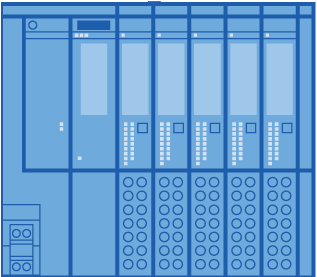
\includegraphics[width=52.5pt,height=52.5pt]{images/siemens_schema.png}};
%Image [id:dp16537534423117606]
\draw (423,74) node  {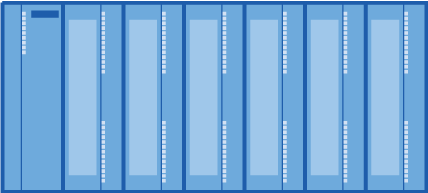
\includegraphics[width=52.5pt,height=25.5pt]{images/entree_sortie_schema.png}};
%Curve Lines [id:da9047126032159685]
\draw [color={rgb, 255:red, 245; green, 166; blue, 35 }  ,draw opacity=1 ]   (278,88) .. controls (279.98,135.52) and (340.52,114.92) .. (386.61,91.7) ;
\draw [shift={(388,91)}, rotate = 513.06] [color={rgb, 255:red, 245; green, 166; blue, 35 }  ,draw opacity=1 ][line width=0.75]    (10.93,-3.29) .. controls (6.95,-1.4) and (3.31,-0.3) .. (0,0) .. controls (3.31,0.3) and (6.95,1.4) .. (10.93,3.29)   ;

%Rounded Rect [id:dp33312095954877385]
\draw   (381,128.03) .. controls (381,123.59) and (384.59,120) .. (389.03,120) -- (454.57,120) .. controls (459.01,120) and (462.6,123.59) .. (462.6,128.03) -- (462.6,152.11) .. controls (462.6,156.54) and (459.01,160.13) .. (454.57,160.13) -- (389.03,160.13) .. controls (384.59,160.13) and (381,156.54) .. (381,152.11) -- cycle ;
%Straight Lines [id:da4805908792581848]
\draw [color={rgb, 255:red, 65; green, 117; blue, 5 }  ,draw opacity=1 ]   (405,91) -- (405,118) ;
\draw [shift={(405,120)}, rotate = 270] [color={rgb, 255:red, 65; green, 117; blue, 5 }  ,draw opacity=1 ][line width=0.75]    (10.93,-3.29) .. controls (6.95,-1.4) and (3.31,-0.3) .. (0,0) .. controls (3.31,0.3) and (6.95,1.4) .. (10.93,3.29)   ;

%Straight Lines [id:da046732551722878934]
\draw [color={rgb, 255:red, 208; green, 2; blue, 27 }  ,draw opacity=1 ]   (400,120) -- (400,93) ;
\draw [shift={(400,91)}, rotate = 450] [color={rgb, 255:red, 208; green, 2; blue, 27 }  ,draw opacity=1 ][line width=0.75]    (10.93,-3.29) .. controls (6.95,-1.4) and (3.31,-0.3) .. (0,0) .. controls (3.31,0.3) and (6.95,1.4) .. (10.93,3.29)   ;

%Straight Lines [id:da5001732327017756]
\draw [color={rgb, 255:red, 65; green, 117; blue, 5 }  ,draw opacity=1 ]   (438,91) -- (438,118) ;
\draw [shift={(438,120)}, rotate = 270] [color={rgb, 255:red, 65; green, 117; blue, 5 }  ,draw opacity=1 ][line width=0.75]    (10.93,-3.29) .. controls (6.95,-1.4) and (3.31,-0.3) .. (0,0) .. controls (3.31,0.3) and (6.95,1.4) .. (10.93,3.29)   ;

%Straight Lines [id:da6761611930473217]
\draw [color={rgb, 255:red, 208; green, 2; blue, 27 }  ,draw opacity=1 ]   (433,120) -- (433,93) ;
\draw [shift={(433,91)}, rotate = 450] [color={rgb, 255:red, 208; green, 2; blue, 27 }  ,draw opacity=1 ][line width=0.75]    (10.93,-3.29) .. controls (6.95,-1.4) and (3.31,-0.3) .. (0,0) .. controls (3.31,0.3) and (6.95,1.4) .. (10.93,3.29)   ;


%Straight Lines [id:da5215523224998694]
\draw [color={rgb, 255:red, 65; green, 117; blue, 5 }  ,draw opacity=1 ]   (422.5,91) -- (422.5,118) ;
\draw [shift={(422.5,120)}, rotate = 270] [color={rgb, 255:red, 65; green, 117; blue, 5 }  ,draw opacity=1 ][line width=0.75]    (10.93,-3.29) .. controls (6.95,-1.4) and (3.31,-0.3) .. (0,0) .. controls (3.31,0.3) and (6.95,1.4) .. (10.93,3.29)   ;

%Straight Lines [id:da15501163618778613]
\draw [color={rgb, 255:red, 208; green, 2; blue, 27 }  ,draw opacity=1 ]   (417.5,120) -- (417.5,93) ;
\draw [shift={(417.5,91)}, rotate = 450] [color={rgb, 255:red, 208; green, 2; blue, 27 }  ,draw opacity=1 ][line width=0.75]    (10.93,-3.29) .. controls (6.95,-1.4) and (3.31,-0.3) .. (0,0) .. controls (3.31,0.3) and (6.95,1.4) .. (10.93,3.29)   ;




% Text Node
\draw (304,126) node [scale=0.9,color={rgb, 255:red, 245; green, 166; blue, 35 }  ,opacity=1 ] [align=left] {Bus de terrain};
% Text Node
\draw (421.8,140.07) node  [align=left] {Système};


\end{tikzpicture}

	\caption{Strucure distribuée}
	\end{subfigure}
	\caption{Schéma de structure locale et déportée}
	\label{fig:local_deporte}
\end{figure}

Les bus de terrain reliant les modules peuvent être de différentes natures selon la configuration (CAN, Profibus, LON, BACNET, Ethernet, \dots).

\UPSTIaRetenir{%
\begin{description}
	\item [Sructure locale : ] Les modules d'entrées et de sorties sont reliées directements à l'automate.
	\item [Strucure déportée : ] Les modules d'entrées et de sorties sont déportées proches des capteurs et actionneurs et communiquent avec l'automates à l'aide d'un BUS de terrain.
\end{description}
}
